\documentclass{beamer}
\usepackage[utf8]{inputenc}
\usepackage[T1]{fontenc}
\usepackage[polish]{babel}
\usepackage{graphicx}
\usepackage{amsmath}

\usetheme{Madrid}

% Definiujemy własny kolor w formacie RGB (Red, Green, Blue od 0 do 255)
\definecolor{CiemnyCzerwony}{RGB}{139,0,0} 

% Przypisujemy go jako główny kolor prezentacji
\setbeamercolor{structure}{fg=CiemnyCzerwony}

\title{Podstawy Rachunku Prawdopodobieństwa}
\author{Imię i Nazwisko}
\date{\today}

\begin{document}

% Slajd 1: Tytułowy
\begin{frame}
\titlepage
\end{frame}

% Slajd 2: Spis treści
\begin{frame}{Spis treści}
\tableofcontents
\end{frame}

\section{Podstawowe pojęcia}

% Slajd 3
\begin{frame}{1. Przestrzeń zdarzeń elementarnych}
\begin{itemize}
    \item Zbiór wszystkich możliwych wyników doświadczenia losowego oznaczamy literą $\Omega$.
    \item Elementy tego zbioru nazywamy zdarzeniami elementarnymi (ozn. $\omega$).
\end{itemize}
\begin{block}{Definicja}
Zdarzeniem losowym $A$ nazywamy dowolny podzbiór przestrzeni $\Omega$, czyli $A \subseteq \Omega$.
\end{block}
\end{frame}

\section{Definicje prawdopodobieństwa}

% Slajd 4
\begin{frame}{2. Klasyczna definicja prawdopodobieństwa}
Jeśli $\Omega$ jest zbiorem skończonym, a wszystkie zdarzenia elementarne są jednakowo prawdopodobne, to prawdopodobieństwo zdarzenia $A$ wyraża się wzorem:
\begin{equation}
P(A) = \frac{|A|}{|\Omega|}
\end{equation}
Gdzie:
\begin{enumerate}
    \item $|A|$ to liczba zdarzeń sprzyjających zdarzeniu $A$,
    \item $|\Omega|$ to liczba wszystkich możliwych zdarzeń elementarnych.
\end{enumerate}
\end{frame}

% Slajd 5
\begin{frame}{3. Aksjomatyczna definicja Kołmogorowa}
Prawdopodobieństwo to funkcja $P: \mathcal{F} \to [0,1]$ spełniająca warunki:
\begin{itemize}
    \item $P(A) \ge 0$ dla każdego zdarzenia $A$,
    \item $P(\Omega) = 1$ (prawdopodobieństwo zdarzenia pewnego),
    \item Dla ciągu parami rozłącznych zdarzeń $A_1, A_2, \dots$:
\end{itemize}
\begin{equation}
P\left(\bigcup_{i=1}^\infty A_i\right) = \sum_{i=1}^\infty P(A_i)
\end{equation}
\end{frame}

\section{Zależności między zdarzeniami}

% Slajd 6
\begin{frame}{4. Prawdopodobieństwo warunkowe}
\begin{exampleblock}{Przykład}
Rzucamy dwiema kostkami. Jakie jest prawdopodobieństwo wyrzucenia sumy oczek 8, jeśli wiemy, że na pierwszej kostce wypadło 5?
\end{exampleblock}
Wzór na prawdopodobieństwo zdarzenia $A$ pod warunkiem $B$ (gdzie $P(B)>0$):
\begin{equation}
P(A|B) = \frac{P(A \cap B)}{P(B)}
\end{equation}
\end{frame}

% Slajd 7
\begin{frame}{5. Niezależność zdarzeń}
Dwa zdarzenia $A$ i $B$ nazywamy niezależnymi, jeśli:
\begin{equation}
P(A \cap B) = P(A) \cdot P(B)
\end{equation}
\vspace{0.5cm}
\begin{alertblock}{Uwaga!}
Niezależność zdarzeń to nie to samo co ich rozłączność ($A \cap B = \emptyset$). Rozłączne zdarzenia o dodatnim prawdopodobieństwie są zawsze zależne!
\end{alertblock}
\end{frame}

% Slajd 8
\begin{frame}{6. Prawdopodobieństwo całkowite i Wzór Bayesa}
Jeśli zdarzenia $B_1, B_2, \dots, B_n$ tworzą podział przestrzeni $\Omega$, to:
\begin{equation}
P(A) = \sum_{i=1}^n P(A|B_i)P(B_i)
\end{equation}
Wzór Bayesa pozwala na "odwrócenie" prawdopodobieństwa warunkowego:
\begin{block}{Twierdzenie Bayesa}
\begin{equation}
P(B_k|A) = \frac{P(A|B_k)P(B_k)}{\sum_{i=1}^n P(A|B_i)P(B_i)}
\end{equation}
\end{block}
\end{frame}

\section{Zmienne losowe}

% Slajd 9 (Kolumny)
\begin{frame}{7. Parametry zmiennej losowej}
\begin{columns}
\column{0.5\textwidth}
\textbf{Wartość oczekiwana} $\mathbb{E}X$
\begin{itemize}
    \item Miara przeciętnego położenia
    \item Dla zmiennej dyskretnej: \\ $\mathbb{E}X = \sum_{i} x_i p_i$
\end{itemize}

\column{0.5\textwidth}
\textbf{Wariancja} $Var(X)$
\begin{itemize}
    \item Miara rozrzutu wokół średniej
    \item $Var(X) = \mathbb{E}(X - \mathbb{E}X)^2$
    \item $Var(X) = \mathbb{E}(X^2) - (\mathbb{E}X)^2$
\end{itemize}
\end{columns}
\end{frame}

% Slajd 10 (Obrazek)
\begin{frame}{8. Rozkład normalny (Krzywa Gaussa)}
Gęstość rozkładu normalnego opisana jest wzorem:
\begin{equation*}
f(x) = \frac{1}{\sigma \sqrt{2\pi}} e^{-\frac{(x-\mu)^2}{2\sigma^2}}
\end{equation*}

\vspace{0.5cm}
\begin{center}
% ABY DODAĆ PRAWDZIWY OBRAZEK: 
% 1. Wgraj plik (np. "wykres.png") do Overleafa (przycisk Upload)
% 2. Usuń komendę \framebox poniżej
% 3. Odkomentuj (usuń znak %) z linijki z \includegraphics
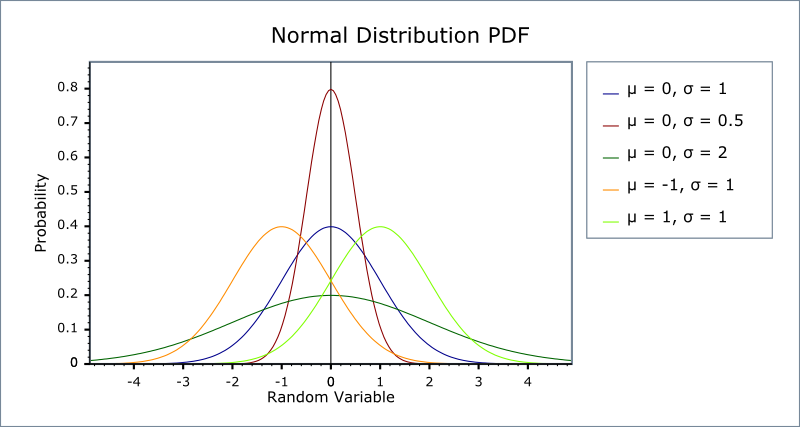
\includegraphics[width=0.9\textwidth]{normal_pdf.png}
\end{center}
\end{frame}

\end{document}